\documentclass{sigplanconf} %[10pt]

\usepackage[utf8]{inputenc}
\usepackage[T1]{fontenc}
\usepackage{listings}
\usepackage{xcolor}
\usepackage{hyperref}
\usepackage{graphics}
\usepackage{array} % tables
\usepackage{afterpage} % figures
\usepackage{float} % figures
\usepackage{paralist} % figures
\usepackage[shortcuts]{extdash} % figures
\usepackage{todonotes}
\usepackage{textcomp}
% \usepackage{lmodern}
\usepackage{multirow}
\usepackage{ctable}
\usepackage{relsize}
\usepackage{amsmath,amssymb}
\usepackage{siunitx}
 \sisetup{
    binary-units,
    detect-all,
    free-standing-units,
    space-before-unit,
    use-xspace,
    unit-optional-argument,
    parse-units = false,
  }
%\usepackage[scaled=0.9]{inconsolata}
\usepackage[scaled=0.85]{beramono}
\usepackage[final]{microtype}
\microtypesetup{stretch=9,shrink=15,step=3,letterspace=50}
% % Disable single lines at the start of a paragraph (Schusterjungen)
% \clubpenalty = 10000
% % Disable single lines at the end of a paragraph (Hurenkinder)
% \widowpenalty = 10000 
% \displaywidowpenalty = 10000 % formulas

\usepackage[pass,letterpaper]{geometry}

\usepackage{balance}
\usepackage{subcaption}

\providecommand*{\lstnumberautorefname}{line}
\providecommand*{\lstlistingautorefname}{listing}

\begin{document}

\providecommand*\hairspace{\ifmmode\mskip1mu\else\kern0.08em\fi}
\providecommand*\eg{e.\hairspace{}g.\xspace}
\providecommand*\Eg{E.\hairspace{}g.\xspace}
\providecommand*\Ie{I.\hairspace{}e.\xspace}
\providecommand*\ie{i.\hairspace{}e.\xspace}

\nocaptionrule

\newenvironment{Compactenum}
{\setlength{\leftmargini}{1em}
\begin{enumerate}
  \setlength{\labelsep}{.3em}
  \setlength{\itemsep}{.4em}
  \setlength{\parskip}{0pt}
  \setlength{\parsep}{0pt}}
{\end{enumerate}}

% Define our own compact itemize
\newenvironment{Compactitem}
{\setlength{\leftmargini}{1em}
\begin{itemize}
  \setlength{\labelsep}{.3em}
  \setlength{\itemsep}{.4em}
  \setlength{\parskip}{0pt}
  \setlength{\parsep}{0pt}}
{\end{itemize}}

\lstset{language=Ruby,
% backgroundcolor=\color[rgb]{0.95, 0.95, 0.95},
tabsize=2,
rulecolor=,
basicstyle=\ttfamily,
upquote=true,
% aboveskip={1.5\baselineskip},
columns=fullflexible,
% columns=fixed,
showstringspaces=false,
extendedchars=true,
breaklines=true,
prebreak = \raisebox{0ex}[0ex][0ex]{\ensuremath{\hookleftarrow}},
% frame=single,
showtabs=false,
showspaces=false,
showstringspaces=false,
% identifierstyle=\ttfamily,
keywordstyle=\color[rgb]{1.0,0,0},
keywordstyle=[1]\color[rgb]{0,0,0.75},
keywordstyle=[2]\color[rgb]{0.5,0.0,0.0},
keywordstyle=[3]\color[rgb]{0.127,0.427,0.514},
keywordstyle=[4]\color[rgb]{0.4,0.4,0.4},
commentstyle=\color[rgb]{0.5,0.5,0.5},
stringstyle=\color[rgb]{0.639,0.082,0.082},
morekeywords={self, proceed},
numbers=left,%
numbersep=5pt,%
numberstyle=\tiny\color{gray},%
emphstyle=\bfseries,%
breaklines=true,
breakatwhitespace=true,%
escapechar=`,
}

% \special{papersize=8.5in,11in}
% \setlength{\pdfpageheight}{\paperheight}
% \setlength{\pdfpagewidth}{\paperwidth}

\conferenceinfo{ICOOOLPS '15}{July 6, 2015, Prague, Czech Republic} 
\copyrightyear{2015} 
\copyrightdata{978-1-nnnn-nnnn-n/yy/mm} 
\doi{nnnnnnn.nnnnnnn}

% Uncomment one of the following two, if you are not going for the 
% traditional copyright transfer agreement.

\exclusivelicense                % ACM gets exclusive license to publish, 
                                  % you retain copyright

%\permissiontopublish             % ACM gets nonexclusive license to publish
                                  % (paid open-access papers, 
                                  % short abstracts)

\titlebanner{banner above paper title}        % These are ignored unless
\preprintfooter{short description of paper}   % 'preprint' option specified.

\title{Call-target-specific Method Arguments}
%\subtitle{Subtitle Text, if any}

\authorinfo{Fabio Niephaus \and Matthias Springer \and Tim Felgentreff \and Tobias Pape \and Robert Hirschfeld}
           {Software Architecture Group, Hasso Plattner Institute, University of Potsdam}
           {\{fabio.niephaus, matthias.springer\}@student.hpi.uni-potsdam.de \and \\ \{tim.felgentreff, tobias.pape, hirschfeld\}@hpi.uni-potsdam.de}

\maketitle

\begin{abstract}
Most efficient implementations of dynamically-typed programming languages use polymorphic inline caches to determine the target of polymorphic method calls, making method lookups more efficient. In some programming languages, parameters specified in method signatures can differ from arguments passed at call sites. However, arguments are typically specific to call sites, so they have to be converted in target methods. We propose call-target-specific method arguments for dynamically-typed languages, effectively making argument handling part of polymorphic inline cache entries. We implemented this concept in JRuby using the Truffle framework in order to make keyword arguments more efficient. Micro-benchmarks confirm that our implementation makes keyword argument passing in JRuby more than twice as fast.
\end{abstract}

% A category with the (minimum) three required fields
%\category{H.4}{Information Systems Applications}{Miscellaneous}
%A category including the fourth, optional field follows...
%\category{D.2.8}{Software Engineering}{Metrics}[complexity measures, performance measures]

%\category{CR-number}{subcategory}{third-level}
 % A category with the (minimum) three required fields
 \category{D.1.5}{Programming Techniques}{Object-Oriented Programming}
 %A category including the fourth, optional field follows...
 \category{D.3.4}{Programming Languages}{Processors}[code generation, optimization]

% general terms are not compulsory anymore, 
% you may leave them out
% \terms
% Languages, Virtual Machines, Performance

\keywords
PIC, Method Arguments, Named Arguments, JRuby %, Truffle

\section{Introduction}
Dynamically-typed object-oriented programming languages typically use polymorphic inline caches~\cite{Holzle:1991:ODO:646149.679193} during method dispatch to find the corresponding target method quickly: a small number of class types is stored along with method pointers at every call site. In some programming languages, however, different call targets that are cached by the same call site can require different arguments: Ruby keyword arguments will serve as a running example in this paper and are introduced in Section~\ref{sec:kwargs}. 

The main contribution of this paper are \emph{call-target-specific method arguments}: instead of converting arguments into a call-site-specific format and sharing them among all call targets, our approach aims to make method arguments call-target-specific. Based on the polymorphic type of the receiver, the call site directly converts the arguments to the method-specific format. Call-target-specific method arguments were designed for dynamically-typed programming languages; a different idea has been proposed and implemented for statically-typed programming languages and is presented briefly in Section~\ref{sec:related}.

\section{Example: Ruby Keyword Arguments}
\label{sec:kwargs}
Keyword arguments (named arguments) in Ruby will serve as a running example in the remainder of this paper, but other constructs~\cite{Zdun05patternsof} such as variable-sized argument lists with a rest argument are amenable to our approach. The usage of keyword arguments is wide-spread in Ruby: for instance, libraries like \emph{ActiveRecord} typically pass optional \lstinline{options} arguments as keyword arguments. Ruby 2.0 introduced a more compact syntax for keyword arguments (Listing~1), in addition to the old syntax. 

\begin{figure}[!hbp] %,label=fig:ruby_kwargs,caption=Example usage of keyword arguments in Ruby.]
\begin{lstlisting}[basicstyle=\footnotesize\ttfamily] 
def A.foo(a:, b:)
   a + b
end

def B.foo(b:, a:)
   a + b
end

def C.foo(a:, **kwargs) `\label{lst:kwargs}`
   a + kwargs[:b]
end

object.foo(a: 1, b: 2) `\label{lst:invocation}`
object.foo({a: 1, b: 2})  `\label{lst:invocation2}`
\end{lstlisting}
\vspace{-0.25cm}
\caption*{Listing 1: Example usage of keyword arguments in Ruby.}
\end{figure}

Keyword arguments are named arguments. The order in which they are passed in a method call does not matter. Excess keyword arguments are available as a dictionary (``hash'' in Ruby) in the target method's body (\lstinline{**kwargs} in \autoref{lst:kwargs}) or cause an argument error if no such \emph{rest keyword parameter} is defined in the method's signature.

Whenever keyword arguments are passed at a call site, both MRI\footnote{MRI (Matz's Ruby Interpreter) is the Ruby reference implementation.} and JRuby store all keyword arguments in a dictionary and use that dictionary as the last argument. Whenever a keyword argument is present in a method's signature, the method checks if the last argument is a dictionary, extracts the corresponding keyword argument from the dictionary and stores it in a temporary variable.

When executing \autoref{lst:invocation}, Ruby first creates a dictionary containing all keyword arguments (``representation that is compatible with all call targets'') and then extracts keyword arguments mentioned in the method signature again (``method-specific representation'').

% Running example: Ruby Keyword Arguments + Truffle

\section{Call-target-specific Arguments}
In this section, we explain how our solution is different from existing programming language implementations on a more abstract level. A language implementation typically performs the following steps when calling a method.

\begin{Compactenum}
       \item Convert arguments into a (generic) representation which is compatible with all call targets (\eg create a dictionary containing all keyword arguments).
       \item Push arguments on stack.
       \item Look target method up (possibly using PIC).
       \item Dispatch to target method.
       \item Convert arguments to method-specific representation (\eg extract keyword arguments mentioned in the method signature from the dictionary).
       \item Execute method body.
\end{Compactenum}

\autoref{fig:pic_abstr} shows polymorphic inline caches for call sites A and B with call-site-specific method arguments (a) and call-target-specific method arguments (b). In the former case, the exact same generic arguments are passed to all target methods for a specific call site. In the latter case, different arguments can be passed to target methods.
%\begin{figure}
%        \centering
%        \subfloat[call-site-specific targets]{
\includegraphics[width=0.45\linewidth]{resources/class_call_site}} 
%        \hfill
%        \subfloat[call-target-specific sites]{\includegraphics[width=0.45\linewidth]{resources/class_call_target}} \\
%        \subfloat[Adapter (shared representation)]{
\includegraphics[width=0.9\linewidth]{resources/class_adapter}} 
%    \caption{Polymorphic inline cache for method dispatch.}
%    \label{fig:pic_abstr}
%\end{figure}

\begin{figure}[!htp]
        \centering
        \begin{subfigure}{.45\linewidth}
          
\includegraphics[width=.9\linewidth]{resources/pic_regular}
          \caption{Without call-target-specific arguments}
        \end{subfigure}
        \hfill
        \begin{subfigure}{.45\linewidth}
          
\includegraphics[width=.9\linewidth]{resources/pic_calltarget}
          \caption{Without call-target-specific arguments}
        \end{subfigure}
    \caption{Polymorphic inline cache for method dispatch.}
    \label{fig:pic_abstr}
\end{figure}

Although every call site along with its arguments is represented by a single statement in the source code (\eg Listing~1, \autoref{lst:invocation}), the execution environment might decide to pass different arguments for every polymorphic target type.

Polymorphic inline caches avoid unnecessary method lookups by caching call target methods for receiver types. Call-target-specific method arguments make argument handling more efficient by avoiding generic argument representations.

\section{Implementation}
In this section, we present our proof-of-concept implementation in JRuby. JRuby is an implementation of the Ruby programming language in Java and uses Truffle, an AST interpreter framework for AST node rewriting and partial evaluation (inlining)~\cite{Wurthinger:2013:OVR:2509578.2509581, Wurthinger:2012:SAI:2384577.2384587}. Truffle runs on top of the Graal virtual machine~\cite{Wimmer:2012:TSR:2384716.2384723}, a modified HotSpot virtual machine, that provides runtime feedback to Truffle and can compile and install new optimized code on the fly.

\subsection{JRuby Keyword Arguments}
\autoref{fig:pic_jruby} shows JRuby's implementation of polymorphic inline
caches (\emph{type decision chains}) for a call site. Initially, for the
\lstinline{CallDispatchHeadNode} no target method is cached so far, so it has a reference to an \lstinline{UnresolvedDispatchNode} object. Upon successful method lookup, this reference is replaced by a reference to a \lstinline{CachedDispatchNode} object, representing an entry in the polymorphic inline cache. That object has a reference to the next cache entry, which is initially an \lstinline{UncachedDispatchNode} object but can be replaced by another cache entry, forming a linked list of cache entries. This list of cache entries is replaced by an \lstinline{UncachedDispatchNode} object once the length of the list exceeds a threshold value, falling back to regular method lookup.

\begin{figure*}
        \centering
        \begin{subfigure}{.48\linewidth}
          \centering
          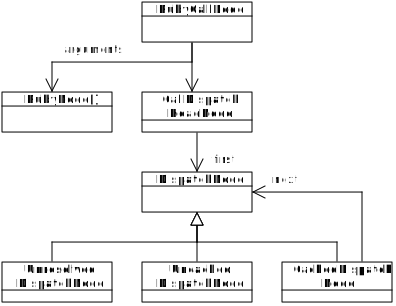
\includegraphics[width=.75\linewidth]{resources/dispatch}
          \caption{Call-site-specific}
        \end{subfigure}
        \hspace{1em}
        \begin{subfigure}{.48\linewidth}
          \centering
          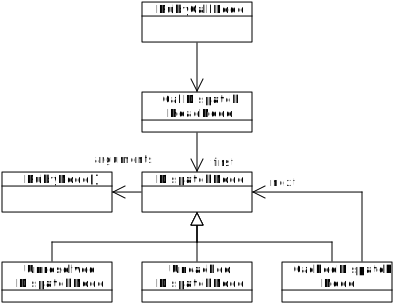
\includegraphics[width=.75\linewidth]{resources/dispatch_opt}
          \caption{Call-target-specific}
        \end{subfigure}
    \caption{Polymorphic inline caching and argument AST nodes in JRuby with Truffle.}
    \label{fig:pic_jruby}
\end{figure*}

The original JRuby implementation stores the array of AST nodes for method arguments in \lstinline{RubyCallNode}, which is specific to a certain call site. Our optimization stores method arguments in \lstinline{DispatchNode} which is specific to a certain call target. Upon creation of PIC entries, our implementation analyzes the target method and stores AST nodes in the array of arguments in such a way that the $i$\textsuperscript{th} argument in the method signature corresponds to the $i$\textsuperscript{th} argument in the array, making it easy to load arguments within the target method without having to extract arguments from a dictionary.

\paragraph{Example}
Consider the case that \autoref{lst:invocation} in Listing~1 is executed multiple times, but \lstinline{object} alternates between instances of \lstinline{A}, \lstinline{B}, and \lstinline{C}. Our implementation generates three different argument arrays that are specific to one of the three \lstinline{foo} methods\footnote{For better readability, we use Ruby syntax. Since the arguments array is part of the AST, all objects should be AST nodes (fixnum literal nodes, symbol literal nodes and hash literal nodes). Marker nodes are omitted.}.
\begin{Compactitem}
       \item \lstinline|A.foo: [1, 2]|
       \item \lstinline|B.foo: [2, 1]|
       \item \lstinline|C.foo: [1, {:b => 2}]|
\end{Compactitem}

\paragraph{Pitfalls and Implementation Details}
In Ruby, keyword arguments can be passed explicitly as named arguments (Listing~1, \autoref{lst:invocation}) and implicitly using an already existing dictionary object (Listing~2, \autoref{lst:invocation2}). The latter case cannot be optimized by expanding dictionaries. Therefore, the original implementation should stay in place for this case.

Target methods must be able to distinguish whether the arguments of the current invocation are optimized (expanded) or not. We use a special marker object (Figure~\ref{fig:rubyarr}) at the end of the arguments array to denote that a call is optimized and keyword arguments can be read from the array directly without looking them up in a dictionary.

\begin{figure}[!htp]

\includegraphics[width=\linewidth]{resources/rubyargs}
\caption{Ruby arguments array during method dispatch in JRuby.}
\label{fig:rubyarr}
\end{figure}

Since we might rearrange AST nodes in the arguments array, the evaluation order of arguments might have changed. We solve this problem by evaluating arguments in their original order, storing their values into newly-created temporary variables, and passing AST nodes reading the temporary variables, possibly in a different order.

%\subsection{Python Keyword Arguments}
\subsection{Benchmarks}
We ran benchmarks (see Appendix) on our optimized JRuby implementation with Truffle on an ordinary HotSpot VM (no Graal). The benchmarks were run on a MacBook Pro with an i7-2720QM CPU and 16~GB RAM. The benchmarking code and our implementation, along with an install script, is also available for download\footnote{\mbox{\url{https://github.com/HPI-SWA-Lab/TargetSpecific-ICOOOLPS}}.}.

For every benchmark, we compare two implementations: the original, unoptimized implementation of JRuby (\emph{call-site-specific}); and the optimized call-target-specific implementation. In the latter case, a separate AST subtree is stored with every PIC entry\footnote{This is different from Truffle AST node rewriting because multiple AST subtrees can be stored for a call site at the same time.} (an AST subtree generating the array of arguments passed to the target method is stored for every PIC entry).

\begin{figure}[!htp]
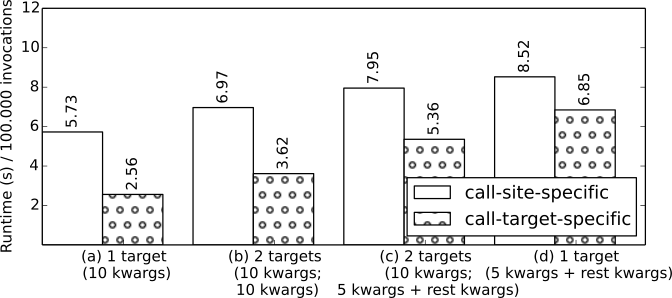
\includegraphics[width=\linewidth]{resources/benchmark}
\caption{Benchmark comparing call-site-specific and call-target-specific method invocation.}
\label{fig:benchmark}
\end{figure}

We benchmarked calling a method on object \lstinline{obj} with 10 keyword arguments (Figure~\ref{fig:benchmark}). In (a) and (d), \lstinline{obj} is always the same object, whereas in (b) and (c), \lstinline{obj} alternates between two objects, whose methods have a different signature. In (a) and (b), the target methods take 10 keyword arguments, whereas in (d), the target methods takes 5 keyword arguments and a rest keyword dictionary. In (c), one of the target methods takes 10 keyword arguments.

Reading a keyword argument from the rest keyword argument hash is slow. That is why (a) is fastest benchmark and (d) is the slowest benchmark.

\section{Related Work}
\label{sec:related}
Named parameters are supported in a wide range of programming languages. For example, Scala supports named arguments which can be optional (``implicit''). Since Scala is a statically-typed programming language, the polymorphic receiver type and, therefore, the target method's signature is known, because methods overridden in subclasses must have the same arguments as the base method. During method application, a collection consisting of all positional arguments followed by a fixed permutation of all named arguments defined in the signature is passed~\cite{Rytz:2010:NDA:1774088.1774529}. Scala evaluates arguments in their original order, stores them in temporary variables, and passes these variables in a permutated order, just as our implementation does. For every optional argument, there is a \emph{default method} (automatically generated in the receiver's class) returning the value of the optional argument. When a method is called with optional arguments missing, the compiler generates code that first calls the corresponding default methods and then passes their return values together with the provided arguments. This is an elegant approach to make argument handling efficient, however, it cannot be applied in dynamically-typed programming languages, because the receiver type of a method call is unknown before dispatching the method call; therefore, the execution environment cannot know if a default argument is missing before looking up the receiver type.

%\lstset{language=Java}
MagLev is an implementation of the Ruby programming language on top of the GemStone/S virtual machine (Smalltalk). For every Ruby method, MagLev generates a set of \emph{bridge methods} specific to a certain number of arguments and splat arguments. When calling a Ruby method, MagLev calls the corresponding bridge method which might provide default arguments and prepare a splat argument array, and calls the actual implementation. For example, if \lstinline{foo(a = 1, *args)} is called via \lstinline{foo(1, 2, 3)}, MagLev calls the bridge method \lstinline{foo#3__} specific to three arguments which wraps the last two arguments in an array and calls the actual implementation~\cite{SprBachelor}. If we extend this idea to keyword arguments, MagLev could also create bridge methods specific to keyword argument labels: whenever a method call with keyword arguments is compiled, MagLev could add a corresponding bridge method to all classes having a method with that name; \eg compiling \lstinline{foo(1, b: 2, a: 1)} could generate bridge methods \lstinline{foo#1__a_b} (one positional argument, keyword arguments \lstinline{a} and \lstinline{b}\footnote{Keyword arguments are sorted lexicographically.}). This would avoid creating and expanding dictionaries when using keyword arguments, but it could also increase the number of methods significantly: in contrast to making arguments call-target-specific, this approach would add call-site-specific wrapper methods.

Gil and Lenza propose an extension of the Java programming language to support keyword arguments and optional arguments~\cite{JOT:issue_2012_04/article1}. Their implementation generates \emph{auxiliary methods} for all valid calling patterns, which is similar to MagLev's concept of bridge methods. Auxiliary methods provide missing arguments and call the actual implementation with the full set of arguments.

In programming languages supporting multiple dispatch, the call target depends on all arguments (usually argument types) instead of just the receiver argument~\cite{multimethods}. Multiple dispatch is used to provide entirely different method implementations for different argument types. Call-target-specific method arguments are, however, an optimization \emph{under the hood}, and aim at making argument handling more efficient, instead of providing different semantics for different argument types.
%TODO: https://www.cs.utah.edu/plt/publications/scheme09-fb.pdf

\section{Conclusion}
We presented call-target-specific method arguments, making method arguments part of polymorphic inline cache entries. Our idea can be used to adapt call sites to do argument conversions a single time whenever a new entry is added to a polymorphic inline cache. When a method call is then executed and the receiver's type was found in the cache, the callee can directly start executing the method body without having to do argument conversions like finding named arguments inside a dictionary.

Future work might investigate how call-target-specific method arguments can be applied to other programming languages. For example, Python supports named arguments which are similar to Ruby's keyword arguments. However, it is unclear to what degree efficient implementations such as PyPy~\cite{Bolz:2009:TMP:1565824.1565827} will benefit from this optimization, since their tracing JIT compiler might already be able to improve the usage of named arguments. PyPy analyzes passed arguments and initializes local variables in stack frames by going through all named arguments (name-value pairs); this iteration step could be omitted at subsequent method calls when using call-target-specific method arguments.

\acks
We would like to thank Chris Seaton for his support with our JRuby implementation.

%\newpage
%
% The following two commands are all you need in the
% initial runs of your .tex file to
% produce the bibliography for the citations in your paper.
\bibliographystyle{abbrvnat}
\bibliography{call_target_specific_method_arguments}  % sigproc.bib is the name of the Bibliography in this case

\appendix
\section{Appendix}
\begin{figure}[!htp]
\begin{lstlisting}[basicstyle=\footnotesize\ttfamily] 
class A
  def foo_a(a:1, b:2, c:3, d:4, e:5, f:6, g:7, h:8, i:9, j:10)
    a + b + c + d + e + f + g + h + i + j
  end

  def foo_b(a:1, b:2, c:3, d:4, e:5, f:6, g:7, h:8, i:9, j:10)
    a + b + c + d + e + f + g + h + i + j
  end

  def foo_c(a:1, b:2, c:3, d:4, e:5, f:6, g:7, h:8, i:9, j:10)
    a + b + c + d + e + f + g + h + i + j
  end
end

class B
  def foo_b(j:11, i:12, h:13, g:14, f:15, e:16, d:17, c:18, b:19, a:20)
    a + b + c + d + e + f + g + h + i + j
  end

  def foo_c(j:11, i:12, h:13, g:14, f:15, **kwargs)
    kwargs[:a] + kwargs[:b] + kwargs[:c] + kwargs[:d] + kwargs[:e] + f + g + h + i + j
  end

  def foo_d(j:11, i:12, h:13, g:14, f:15, **kwargs)
    kwargs[:a] + kwargs[:b] + kwargs[:c] + kwargs[:d] + kwargs[:e] + f + g + h + i + j
  end
end

# Benchmark (a): one target A
obj.foo_a(a:1, b:2, c:3, d:4, e:5, f:6, g:7, h:8, i:9, j:10)

# Benchmark (b): two targets A, B alternating
obj.foo_b(a:1, b:2, c:3, d:4, e:5, f:6, g:7, h:8, i:9, j:10)

# Benchmark (c): two targets A, B alternating
obj.foo_c(a:1, b:2, c:3, d:4, e:5, f:6, g:7, h:8, i:9, j:10)

# Benchmark (d): one target B
obj.foo_d(a:1, b:2, c:3, d:4, e:5, f:6, g:7, h:8, i:9, j:10)
\end{lstlisting}
\caption*{Listing 2: Simplified benchmarking code.}
\end{figure}
%\balance
% You must have a proper ".bib" file
%  and remember to run:
% latex bibtex latex latex
% to resolve all references
%
% ACM needs 'a single self-contained file'!
%
%APPENDICES are optional
%\balancecolumns
\end{document}
